\documentclass[12pt]{article}
\usepackage{tikz}
\usepackage{amsmath}
% Underlining package
\usepackage{ulem}
\usetikzlibrary{calc}
\usepackage[a4paper, portrait, margin=1cm]{geometry}
\usepackage{fancyhdr}

\def \HeadingQuestions {\section*{\Large Name: \underline{\hspace{8cm}} \hfill Date: \underline{\hspace{3cm}}} \vspace{-3mm}
{Angles in a Triangle: Questions} \vspace{1pt}\hrule}

% raise footer with page number; no header
\fancypagestyle{myfancypagestyle}{
  \fancyhf{}% clear all header and footer fields
  \renewcommand{\headrulewidth}{0pt} % no rule under header
  \fancyfoot[C] {\thepage} \setlength{\footskip}{6pt} % raise page number 6pt
}
\pagestyle{myfancypagestyle}  % apply myfancypagestyle

\newcounter{minipagecount}

\begin{document}
\HeadingQuestions
\vspace{8mm}

\begin{minipage}{0.55\textwidth}
  \refstepcounter{minipagecount}
  \noindent{(\theminipagecount)}\quad
  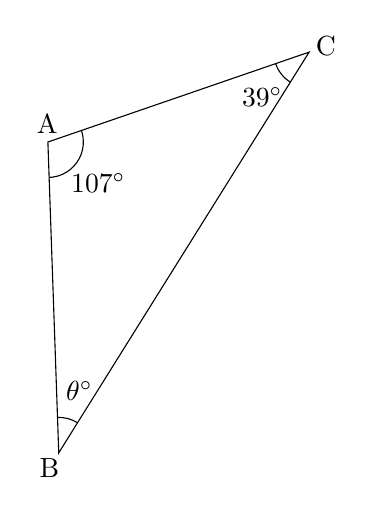
\begin{tikzpicture}[scale=1.5, baseline=(current bounding box.north)]
      \pgfmathsetmacro{\angleA}{34}
      \pgfmathsetmacro{\angleB}{39}
      \pgfmathsetmacro{\angleC}{107}
      \pgfmathsetmacro{\sideC}{4}
      \pgfmathsetmacro{\rotationAngle}{58}
  
    
      \begin{scope}[rotate=\rotationAngle]
        \coordinate (A) at (0,0);
        \coordinate (B) at (\sideC,0);
        \coordinate (C) at (intersection cs: first line={(A)--($(A)+(\angleA:4cm)$)}, second line={(B)--($(B)+(180-\angleB:4cm)$)});
        \draw (A) -- (B) -- (C) -- cycle;
        
        % Mark angles with arcs
        \draw ($(A)!0.3cm!(B)$) arc [start angle=0, end angle=\angleA, radius=0.3cm];
        \draw ($(B)!0.3cm!(C)$) arc [start angle=180-\angleB, end angle=180, radius=0.3cm];
        \draw ($(C)!0.3cm!(A)$) arc [start angle=180+\angleA, end angle=360-\angleB, radius=0.3cm];
        
        % Label angles
        \node at ($(A)!-0.15cm!(B)$) {B};
        \node at ($(B)!-0.15cm!(C)$) {C};
        \node at ($(C)!-0.15cm!(A)$) {A};
        
        % Mark angles in degrees
        \coordinate (midBC) at ($(B)!0.5!(C)$);
        \node at ($(A)!0.55cm!(midBC)$) {$\theta ^\circ$};
    
        \coordinate (midAC) at ($(A)!0.5!(C)$);
        \node at ($(B)!0.55cm!(midAC)$) {39$^\circ$};
    
        \coordinate (midAB) at ($(A)!0.5!(B)$);
        \node at ($(C)!0.55cm!(midAB)$) {107$^\circ$};
      
      \end{scope}
    \end{tikzpicture}
\end{minipage}%
\hfill
\begin{minipage}{0.4\textwidth}
    \begin{align*}
      \angle \text{B} &= 180^\circ - (\angle \text{C} + \angle \text{A}) \\
        &= 180^\circ - (\dotuline{~~~~~~~}^\circ + \dotuline{~~~~~~~}^\circ) \\
        &= 180^\circ - \dotuline{~~~~~~~}^\circ \\
        &= \dotuline{~~~~~~~}^\circ
    \end{align*}
\end{minipage}

\vspace{1cm}\begin{minipage}{0.55\textwidth}
  \refstepcounter{minipagecount}
  \noindent{(\theminipagecount)}\quad
  \begin{tikzpicture}[scale=1.5, baseline=(current bounding box.north)]
      \pgfmathsetmacro{\angleA}{37}
      \pgfmathsetmacro{\angleB}{40}
      \pgfmathsetmacro{\angleC}{103}
      \pgfmathsetmacro{\sideC}{4}
      \pgfmathsetmacro{\rotationAngle}{207}
  
    
      \begin{scope}[rotate=\rotationAngle]
        \coordinate (A) at (0,0);
        \coordinate (B) at (\sideC,0);
        \coordinate (C) at (intersection cs: first line={(A)--($(A)+(\angleA:4cm)$)}, second line={(B)--($(B)+(180-\angleB:4cm)$)});
        \draw (A) -- (B) -- (C) -- cycle;
        
        % Mark angles with arcs
        \draw ($(A)!0.3cm!(B)$) arc [start angle=0, end angle=\angleA, radius=0.3cm];
        \draw ($(B)!0.3cm!(C)$) arc [start angle=180-\angleB, end angle=180, radius=0.3cm];
        \draw ($(C)!0.3cm!(A)$) arc [start angle=180+\angleA, end angle=360-\angleB, radius=0.3cm];
        
        % Label angles
        \node at ($(A)!-0.15cm!(B)$) {L};
        \node at ($(B)!-0.15cm!(C)$) {M};
        \node at ($(C)!-0.15cm!(A)$) {N};
        
        % Mark angles in degrees
        \coordinate (midBC) at ($(B)!0.5!(C)$);
        \node at ($(A)!0.55cm!(midBC)$) {$\theta ^\circ$};
    
        \coordinate (midAC) at ($(A)!0.5!(C)$);
        \node at ($(B)!0.55cm!(midAC)$) {40$^\circ$};
    
        \coordinate (midAB) at ($(A)!0.5!(B)$);
        \node at ($(C)!0.55cm!(midAB)$) {103$^\circ$};
      
      \end{scope}
    \end{tikzpicture}
\end{minipage}%
\hfill
\begin{minipage}{0.4\textwidth}
    \begin{align*}
      \angle \text{L} &= 180^\circ - (\angle \text{M} + \angle \text{N}) \\
        &= 180^\circ - (\dotuline{~~~~~~~}^\circ + \dotuline{~~~~~~~}^\circ) \\
        &= 180^\circ - \dotuline{~~~~~~~}^\circ \\
        &= \dotuline{~~~~~~~}^\circ
    \end{align*}
\end{minipage}

\vspace{1cm}\begin{minipage}{0.55\textwidth}
  \refstepcounter{minipagecount}
  \noindent{(\theminipagecount)}\quad
  \begin{tikzpicture}[scale=1.5, baseline=(current bounding box.north)]
      \pgfmathsetmacro{\angleA}{32}
      \pgfmathsetmacro{\angleB}{64}
      \pgfmathsetmacro{\angleC}{84}
      \pgfmathsetmacro{\sideC}{4}
      \pgfmathsetmacro{\rotationAngle}{112}
  
    
      \begin{scope}[rotate=\rotationAngle]
        \coordinate (A) at (0,0);
        \coordinate (B) at (\sideC,0);
        \coordinate (C) at (intersection cs: first line={(A)--($(A)+(\angleA:4cm)$)}, second line={(B)--($(B)+(180-\angleB:4cm)$)});
        \draw (A) -- (B) -- (C) -- cycle;
        
        % Mark angles with arcs
        \draw ($(A)!0.3cm!(B)$) arc [start angle=0, end angle=\angleA, radius=0.3cm];
        \draw ($(B)!0.3cm!(C)$) arc [start angle=180-\angleB, end angle=180, radius=0.3cm];
        \draw ($(C)!0.3cm!(A)$) arc [start angle=180+\angleA, end angle=360-\angleB, radius=0.3cm];
        
        % Label angles
        \node at ($(A)!-0.15cm!(B)$) {Y};
        \node at ($(B)!-0.15cm!(C)$) {Z};
        \node at ($(C)!-0.15cm!(A)$) {X};
        
        % Mark angles in degrees
        \coordinate (midBC) at ($(B)!0.5!(C)$);
        \node at ($(A)!0.55cm!(midBC)$) {$\theta ^\circ$};
    
        \coordinate (midAC) at ($(A)!0.5!(C)$);
        \node at ($(B)!0.55cm!(midAC)$) {64$^\circ$};
    
        \coordinate (midAB) at ($(A)!0.5!(B)$);
        \node at ($(C)!0.55cm!(midAB)$) {84$^\circ$};
      
      \end{scope}
    \end{tikzpicture}
\end{minipage}%
\hfill
\begin{minipage}{0.4\textwidth}
    \begin{align*}
      \angle \text{Y} &= 180^\circ - (\angle \text{Z} + \angle \text{X}) \\
        &= 180^\circ - (\dotuline{~~~~~~~}^\circ + \dotuline{~~~~~~~}^\circ) \\
        &= 180^\circ - \dotuline{~~~~~~~}^\circ \\
        &= \dotuline{~~~~~~~}^\circ
    \end{align*}
\end{minipage}

\vspace{1cm}\begin{minipage}{0.55\textwidth}
  \refstepcounter{minipagecount}
  \noindent{(\theminipagecount)}\quad
  \begin{tikzpicture}[scale=1.5, baseline=(current bounding box.north)]
      \pgfmathsetmacro{\angleA}{56}
      \pgfmathsetmacro{\angleB}{64}
      \pgfmathsetmacro{\angleC}{60}
      \pgfmathsetmacro{\sideC}{3}
      \pgfmathsetmacro{\rotationAngle}{215}
  
    
      \begin{scope}[rotate=\rotationAngle]
        \coordinate (A) at (0,0);
        \coordinate (B) at (\sideC,0);
        \coordinate (C) at (intersection cs: first line={(A)--($(A)+(\angleA:4cm)$)}, second line={(B)--($(B)+(180-\angleB:4cm)$)});
        \draw (A) -- (B) -- (C) -- cycle;
        
        % Mark angles with arcs
        \draw ($(A)!0.3cm!(B)$) arc [start angle=0, end angle=\angleA, radius=0.3cm];
        \draw ($(B)!0.3cm!(C)$) arc [start angle=180-\angleB, end angle=180, radius=0.3cm];
        \draw ($(C)!0.3cm!(A)$) arc [start angle=180+\angleA, end angle=360-\angleB, radius=0.3cm];
        
        % Label angles
        \node at ($(A)!-0.15cm!(B)$) {D};
        \node at ($(B)!-0.15cm!(C)$) {E};
        \node at ($(C)!-0.15cm!(A)$) {F};
        
        % Mark angles in degrees
        \coordinate (midBC) at ($(B)!0.5!(C)$);
        \node at ($(A)!0.55cm!(midBC)$) {$\theta ^\circ$};
    
        \coordinate (midAC) at ($(A)!0.5!(C)$);
        \node at ($(B)!0.55cm!(midAC)$) {64$^\circ$};
    
        \coordinate (midAB) at ($(A)!0.5!(B)$);
        \node at ($(C)!0.55cm!(midAB)$) {60$^\circ$};
      
      \end{scope}
    \end{tikzpicture}
\end{minipage}%
\hfill
\begin{minipage}{0.4\textwidth}
    \begin{align*}
      \angle \text{D} &= 180^\circ - (\angle \text{E} + \angle \text{F}) \\
        &= 180^\circ - (\dotuline{~~~~~~~}^\circ + \dotuline{~~~~~~~}^\circ) \\
        &= 180^\circ - \dotuline{~~~~~~~}^\circ \\
        &= \dotuline{~~~~~~~}^\circ
    \end{align*}
\end{minipage}

\vspace{1cm}\begin{minipage}{0.55\textwidth}
  \refstepcounter{minipagecount}
  \noindent{(\theminipagecount)}\quad
  \begin{tikzpicture}[scale=1.5, baseline=(current bounding box.north)]
      \pgfmathsetmacro{\angleA}{51}
      \pgfmathsetmacro{\angleB}{63}
      \pgfmathsetmacro{\angleC}{66}
      \pgfmathsetmacro{\sideC}{4}
      \pgfmathsetmacro{\rotationAngle}{73}
  
    
      \begin{scope}[rotate=\rotationAngle]
        \coordinate (A) at (0,0);
        \coordinate (B) at (\sideC,0);
        \coordinate (C) at (intersection cs: first line={(A)--($(A)+(\angleA:4cm)$)}, second line={(B)--($(B)+(180-\angleB:4cm)$)});
        \draw (A) -- (B) -- (C) -- cycle;
        
        % Mark angles with arcs
        \draw ($(A)!0.3cm!(B)$) arc [start angle=0, end angle=\angleA, radius=0.3cm];
        \draw ($(B)!0.3cm!(C)$) arc [start angle=180-\angleB, end angle=180, radius=0.3cm];
        \draw ($(C)!0.3cm!(A)$) arc [start angle=180+\angleA, end angle=360-\angleB, radius=0.3cm];
        
        % Label angles
        \node at ($(A)!-0.15cm!(B)$) {C};
        \node at ($(B)!-0.15cm!(C)$) {A};
        \node at ($(C)!-0.15cm!(A)$) {B};
        
        % Mark angles in degrees
        \coordinate (midBC) at ($(B)!0.5!(C)$);
        \node at ($(A)!0.55cm!(midBC)$) {$\theta ^\circ$};
    
        \coordinate (midAC) at ($(A)!0.5!(C)$);
        \node at ($(B)!0.55cm!(midAC)$) {63$^\circ$};
    
        \coordinate (midAB) at ($(A)!0.5!(B)$);
        \node at ($(C)!0.55cm!(midAB)$) {66$^\circ$};
      
      \end{scope}
    \end{tikzpicture}
\end{minipage}%
\hfill
\begin{minipage}{0.4\textwidth}
    \begin{align*}
      \angle \text{C} &= 180^\circ - (\angle \text{A} + \angle \text{B}) \\
        &= 180^\circ - (\dotuline{~~~~~~~}^\circ + \dotuline{~~~~~~~}^\circ) \\
        &= 180^\circ - \dotuline{~~~~~~~}^\circ \\
        &= \dotuline{~~~~~~~}^\circ
    \end{align*}
\end{minipage}

\vspace{1cm}\begin{minipage}{0.55\textwidth}
  \refstepcounter{minipagecount}
  \noindent{(\theminipagecount)}\quad
  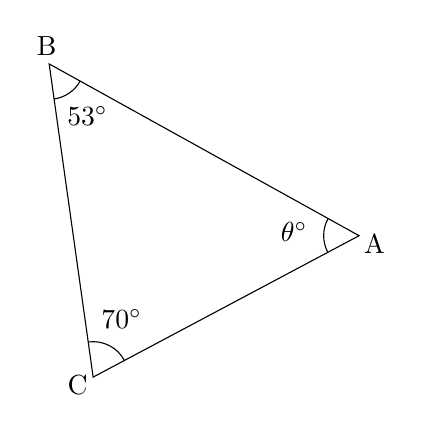
\begin{tikzpicture}[scale=1.5, baseline=(current bounding box.north)]
      \pgfmathsetmacro{\angleA}{57}
      \pgfmathsetmacro{\angleB}{53}
      \pgfmathsetmacro{\angleC}{70}
      \pgfmathsetmacro{\sideC}{3}
      \pgfmathsetmacro{\rotationAngle}{151}
  
    
      \begin{scope}[rotate=\rotationAngle]
        \coordinate (A) at (0,0);
        \coordinate (B) at (\sideC,0);
        \coordinate (C) at (intersection cs: first line={(A)--($(A)+(\angleA:4cm)$)}, second line={(B)--($(B)+(180-\angleB:4cm)$)});
        \draw (A) -- (B) -- (C) -- cycle;
        
        % Mark angles with arcs
        \draw ($(A)!0.3cm!(B)$) arc [start angle=0, end angle=\angleA, radius=0.3cm];
        \draw ($(B)!0.3cm!(C)$) arc [start angle=180-\angleB, end angle=180, radius=0.3cm];
        \draw ($(C)!0.3cm!(A)$) arc [start angle=180+\angleA, end angle=360-\angleB, radius=0.3cm];
        
        % Label angles
        \node at ($(A)!-0.15cm!(B)$) {A};
        \node at ($(B)!-0.15cm!(C)$) {B};
        \node at ($(C)!-0.15cm!(A)$) {C};
        
        % Mark angles in degrees
        \coordinate (midBC) at ($(B)!0.5!(C)$);
        \node at ($(A)!0.55cm!(midBC)$) {$\theta ^\circ$};
    
        \coordinate (midAC) at ($(A)!0.5!(C)$);
        \node at ($(B)!0.55cm!(midAC)$) {53$^\circ$};
    
        \coordinate (midAB) at ($(A)!0.5!(B)$);
        \node at ($(C)!0.55cm!(midAB)$) {70$^\circ$};
      
      \end{scope}
    \end{tikzpicture}
\end{minipage}%
\hfill
\begin{minipage}{0.4\textwidth}
    \begin{align*}
      \angle \text{A} &= 180^\circ - (\angle \text{B} + \angle \text{C}) \\
        &= 180^\circ - (\dotuline{~~~~~~~}^\circ + \dotuline{~~~~~~~}^\circ) \\
        &= 180^\circ - \dotuline{~~~~~~~}^\circ \\
        &= \dotuline{~~~~~~~}^\circ
    \end{align*}
\end{minipage}

\vspace{1cm}\begin{minipage}{0.55\textwidth}
  \refstepcounter{minipagecount}
  \noindent{(\theminipagecount)}\quad
  \begin{tikzpicture}[scale=1.5, baseline=(current bounding box.north)]
      \pgfmathsetmacro{\angleA}{33}
      \pgfmathsetmacro{\angleB}{52}
      \pgfmathsetmacro{\angleC}{95}
      \pgfmathsetmacro{\sideC}{4}
      \pgfmathsetmacro{\rotationAngle}{293}
  
    
      \begin{scope}[rotate=\rotationAngle]
        \coordinate (A) at (0,0);
        \coordinate (B) at (\sideC,0);
        \coordinate (C) at (intersection cs: first line={(A)--($(A)+(\angleA:4cm)$)}, second line={(B)--($(B)+(180-\angleB:4cm)$)});
        \draw (A) -- (B) -- (C) -- cycle;
        
        % Mark angles with arcs
        \draw ($(A)!0.3cm!(B)$) arc [start angle=0, end angle=\angleA, radius=0.3cm];
        \draw ($(B)!0.3cm!(C)$) arc [start angle=180-\angleB, end angle=180, radius=0.3cm];
        \draw ($(C)!0.3cm!(A)$) arc [start angle=180+\angleA, end angle=360-\angleB, radius=0.3cm];
        
        % Label angles
        \node at ($(A)!-0.15cm!(B)$) {X};
        \node at ($(B)!-0.15cm!(C)$) {Z};
        \node at ($(C)!-0.15cm!(A)$) {Y};
        
        % Mark angles in degrees
        \coordinate (midBC) at ($(B)!0.5!(C)$);
        \node at ($(A)!0.55cm!(midBC)$) {$\theta ^\circ$};
    
        \coordinate (midAC) at ($(A)!0.5!(C)$);
        \node at ($(B)!0.55cm!(midAC)$) {52$^\circ$};
    
        \coordinate (midAB) at ($(A)!0.5!(B)$);
        \node at ($(C)!0.55cm!(midAB)$) {95$^\circ$};
      
      \end{scope}
    \end{tikzpicture}
\end{minipage}%
\hfill
\begin{minipage}{0.4\textwidth}
    \begin{align*}
      \angle \text{X} &= 180^\circ - (\angle \text{Z} + \angle \text{Y}) \\
        &= 180^\circ - (\dotuline{~~~~~~~}^\circ + \dotuline{~~~~~~~}^\circ) \\
        &= 180^\circ - \dotuline{~~~~~~~}^\circ \\
        &= \dotuline{~~~~~~~}^\circ
    \end{align*}
\end{minipage}

\vspace{1cm}\begin{minipage}{0.55\textwidth}
  \refstepcounter{minipagecount}
  \noindent{(\theminipagecount)}\quad
  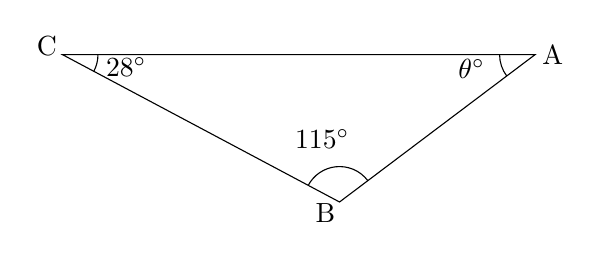
\begin{tikzpicture}[scale=1.5, baseline=(current bounding box.north)]
      \pgfmathsetmacro{\angleA}{37}
      \pgfmathsetmacro{\angleB}{28}
      \pgfmathsetmacro{\angleC}{115}
      \pgfmathsetmacro{\sideC}{4}
      \pgfmathsetmacro{\rotationAngle}{180}
  
    
      \begin{scope}[rotate=\rotationAngle]
        \coordinate (A) at (0,0);
        \coordinate (B) at (\sideC,0);
        \coordinate (C) at (intersection cs: first line={(A)--($(A)+(\angleA:4cm)$)}, second line={(B)--($(B)+(180-\angleB:4cm)$)});
        \draw (A) -- (B) -- (C) -- cycle;
        
        % Mark angles with arcs
        \draw ($(A)!0.3cm!(B)$) arc [start angle=0, end angle=\angleA, radius=0.3cm];
        \draw ($(B)!0.3cm!(C)$) arc [start angle=180-\angleB, end angle=180, radius=0.3cm];
        \draw ($(C)!0.3cm!(A)$) arc [start angle=180+\angleA, end angle=360-\angleB, radius=0.3cm];
        
        % Label angles
        \node at ($(A)!-0.15cm!(B)$) {A};
        \node at ($(B)!-0.15cm!(C)$) {C};
        \node at ($(C)!-0.15cm!(A)$) {B};
        
        % Mark angles in degrees
        \coordinate (midBC) at ($(B)!0.5!(C)$);
        \node at ($(A)!0.55cm!(midBC)$) {$\theta ^\circ$};
    
        \coordinate (midAC) at ($(A)!0.5!(C)$);
        \node at ($(B)!0.55cm!(midAC)$) {28$^\circ$};
    
        \coordinate (midAB) at ($(A)!0.5!(B)$);
        \node at ($(C)!0.55cm!(midAB)$) {115$^\circ$};
      
      \end{scope}
    \end{tikzpicture}
\end{minipage}%
\hfill
\begin{minipage}{0.4\textwidth}
    \begin{align*}
      \angle \text{A} &= 180^\circ - (\angle \text{C} + \angle \text{B}) \\
        &= 180^\circ - (\dotuline{~~~~~~~}^\circ + \dotuline{~~~~~~~}^\circ) \\
        &= 180^\circ - \dotuline{~~~~~~~}^\circ \\
        &= \dotuline{~~~~~~~}^\circ
    \end{align*}
\end{minipage}

\vspace{1cm}\begin{minipage}{0.55\textwidth}
  \refstepcounter{minipagecount}
  \noindent{(\theminipagecount)}\quad
  \begin{tikzpicture}[scale=1.5, baseline=(current bounding box.north)]
      \pgfmathsetmacro{\angleA}{40}
      \pgfmathsetmacro{\angleB}{52}
      \pgfmathsetmacro{\angleC}{88}
      \pgfmathsetmacro{\sideC}{4}
      \pgfmathsetmacro{\rotationAngle}{129}
  
    
      \begin{scope}[rotate=\rotationAngle]
        \coordinate (A) at (0,0);
        \coordinate (B) at (\sideC,0);
        \coordinate (C) at (intersection cs: first line={(A)--($(A)+(\angleA:4cm)$)}, second line={(B)--($(B)+(180-\angleB:4cm)$)});
        \draw (A) -- (B) -- (C) -- cycle;
        
        % Mark angles with arcs
        \draw ($(A)!0.3cm!(B)$) arc [start angle=0, end angle=\angleA, radius=0.3cm];
        \draw ($(B)!0.3cm!(C)$) arc [start angle=180-\angleB, end angle=180, radius=0.3cm];
        \draw ($(C)!0.3cm!(A)$) arc [start angle=180+\angleA, end angle=360-\angleB, radius=0.3cm];
        
        % Label angles
        \node at ($(A)!-0.15cm!(B)$) {R};
        \node at ($(B)!-0.15cm!(C)$) {S};
        \node at ($(C)!-0.15cm!(A)$) {T};
        
        % Mark angles in degrees
        \coordinate (midBC) at ($(B)!0.5!(C)$);
        \node at ($(A)!0.55cm!(midBC)$) {$\theta ^\circ$};
    
        \coordinate (midAC) at ($(A)!0.5!(C)$);
        \node at ($(B)!0.55cm!(midAC)$) {52$^\circ$};
    
        \coordinate (midAB) at ($(A)!0.5!(B)$);
        \node at ($(C)!0.55cm!(midAB)$) {88$^\circ$};
      
      \end{scope}
    \end{tikzpicture}
\end{minipage}%
\hfill
\begin{minipage}{0.4\textwidth}
    \begin{align*}
      \angle \text{R} &= 180^\circ - (\angle \text{S} + \angle \text{T}) \\
        &= 180^\circ - (\dotuline{~~~~~~~}^\circ + \dotuline{~~~~~~~}^\circ) \\
        &= 180^\circ - \dotuline{~~~~~~~}^\circ \\
        &= \dotuline{~~~~~~~}^\circ
    \end{align*}
\end{minipage}

\vspace{1cm}\begin{minipage}{0.55\textwidth}
  \refstepcounter{minipagecount}
  \noindent{(\theminipagecount)}\quad
  \begin{tikzpicture}[scale=1.5, baseline=(current bounding box.north)]
      \pgfmathsetmacro{\angleA}{49}
      \pgfmathsetmacro{\angleB}{46}
      \pgfmathsetmacro{\angleC}{85}
      \pgfmathsetmacro{\sideC}{4}
      \pgfmathsetmacro{\rotationAngle}{78}
  
    
      \begin{scope}[rotate=\rotationAngle]
        \coordinate (A) at (0,0);
        \coordinate (B) at (\sideC,0);
        \coordinate (C) at (intersection cs: first line={(A)--($(A)+(\angleA:4cm)$)}, second line={(B)--($(B)+(180-\angleB:4cm)$)});
        \draw (A) -- (B) -- (C) -- cycle;
        
        % Mark angles with arcs
        \draw ($(A)!0.3cm!(B)$) arc [start angle=0, end angle=\angleA, radius=0.3cm];
        \draw ($(B)!0.3cm!(C)$) arc [start angle=180-\angleB, end angle=180, radius=0.3cm];
        \draw ($(C)!0.3cm!(A)$) arc [start angle=180+\angleA, end angle=360-\angleB, radius=0.3cm];
        
        % Label angles
        \node at ($(A)!-0.15cm!(B)$) {S};
        \node at ($(B)!-0.15cm!(C)$) {R};
        \node at ($(C)!-0.15cm!(A)$) {T};
        
        % Mark angles in degrees
        \coordinate (midBC) at ($(B)!0.5!(C)$);
        \node at ($(A)!0.55cm!(midBC)$) {$\theta ^\circ$};
    
        \coordinate (midAC) at ($(A)!0.5!(C)$);
        \node at ($(B)!0.55cm!(midAC)$) {46$^\circ$};
    
        \coordinate (midAB) at ($(A)!0.5!(B)$);
        \node at ($(C)!0.55cm!(midAB)$) {85$^\circ$};
      
      \end{scope}
    \end{tikzpicture}
\end{minipage}%
\hfill
\begin{minipage}{0.4\textwidth}
    \begin{align*}
      \angle \text{S} &= 180^\circ - (\angle \text{R} + \angle \text{T}) \\
        &= 180^\circ - (\dotuline{~~~~~~~}^\circ + \dotuline{~~~~~~~}^\circ) \\
        &= 180^\circ - \dotuline{~~~~~~~}^\circ \\
        &= \dotuline{~~~~~~~}^\circ
    \end{align*}
\end{minipage}

\vspace{1cm}\begin{minipage}{0.55\textwidth}
  \refstepcounter{minipagecount}
  \noindent{(\theminipagecount)}\quad
  \begin{tikzpicture}[scale=1.5, baseline=(current bounding box.north)]
      \pgfmathsetmacro{\angleA}{27}
      \pgfmathsetmacro{\angleB}{39}
      \pgfmathsetmacro{\angleC}{114}
      \pgfmathsetmacro{\sideC}{4}
      \pgfmathsetmacro{\rotationAngle}{305}
  
    
      \begin{scope}[rotate=\rotationAngle]
        \coordinate (A) at (0,0);
        \coordinate (B) at (\sideC,0);
        \coordinate (C) at (intersection cs: first line={(A)--($(A)+(\angleA:4cm)$)}, second line={(B)--($(B)+(180-\angleB:4cm)$)});
        \draw (A) -- (B) -- (C) -- cycle;
        
        % Mark angles with arcs
        \draw ($(A)!0.3cm!(B)$) arc [start angle=0, end angle=\angleA, radius=0.3cm];
        \draw ($(B)!0.3cm!(C)$) arc [start angle=180-\angleB, end angle=180, radius=0.3cm];
        \draw ($(C)!0.3cm!(A)$) arc [start angle=180+\angleA, end angle=360-\angleB, radius=0.3cm];
        
        % Label angles
        \node at ($(A)!-0.15cm!(B)$) {A};
        \node at ($(B)!-0.15cm!(C)$) {B};
        \node at ($(C)!-0.15cm!(A)$) {C};
        
        % Mark angles in degrees
        \coordinate (midBC) at ($(B)!0.5!(C)$);
        \node at ($(A)!0.55cm!(midBC)$) {$\theta ^\circ$};
    
        \coordinate (midAC) at ($(A)!0.5!(C)$);
        \node at ($(B)!0.55cm!(midAC)$) {39$^\circ$};
    
        \coordinate (midAB) at ($(A)!0.5!(B)$);
        \node at ($(C)!0.55cm!(midAB)$) {114$^\circ$};
      
      \end{scope}
    \end{tikzpicture}
\end{minipage}%
\hfill
\begin{minipage}{0.4\textwidth}
    \begin{align*}
      \angle \text{A} &= 180^\circ - (\angle \text{B} + \angle \text{C}) \\
        &= 180^\circ - (\dotuline{~~~~~~~}^\circ + \dotuline{~~~~~~~}^\circ) \\
        &= 180^\circ - \dotuline{~~~~~~~}^\circ \\
        &= \dotuline{~~~~~~~}^\circ
    \end{align*}
\end{minipage}

\vspace{1cm}\begin{minipage}{0.55\textwidth}
  \refstepcounter{minipagecount}
  \noindent{(\theminipagecount)}\quad
  \begin{tikzpicture}[scale=1.5, baseline=(current bounding box.north)]
      \pgfmathsetmacro{\angleA}{49}
      \pgfmathsetmacro{\angleB}{42}
      \pgfmathsetmacro{\angleC}{89}
      \pgfmathsetmacro{\sideC}{4}
      \pgfmathsetmacro{\rotationAngle}{86}
  
    
      \begin{scope}[rotate=\rotationAngle]
        \coordinate (A) at (0,0);
        \coordinate (B) at (\sideC,0);
        \coordinate (C) at (intersection cs: first line={(A)--($(A)+(\angleA:4cm)$)}, second line={(B)--($(B)+(180-\angleB:4cm)$)});
        \draw (A) -- (B) -- (C) -- cycle;
        
        % Mark angles with arcs
        \draw ($(A)!0.3cm!(B)$) arc [start angle=0, end angle=\angleA, radius=0.3cm];
        \draw ($(B)!0.3cm!(C)$) arc [start angle=180-\angleB, end angle=180, radius=0.3cm];
        \draw ($(C)!0.3cm!(A)$) arc [start angle=180+\angleA, end angle=360-\angleB, radius=0.3cm];
        
        % Label angles
        \node at ($(A)!-0.15cm!(B)$) {T};
        \node at ($(B)!-0.15cm!(C)$) {S};
        \node at ($(C)!-0.15cm!(A)$) {R};
        
        % Mark angles in degrees
        \coordinate (midBC) at ($(B)!0.5!(C)$);
        \node at ($(A)!0.55cm!(midBC)$) {$\theta ^\circ$};
    
        \coordinate (midAC) at ($(A)!0.5!(C)$);
        \node at ($(B)!0.55cm!(midAC)$) {42$^\circ$};
    
        \coordinate (midAB) at ($(A)!0.5!(B)$);
        \node at ($(C)!0.55cm!(midAB)$) {89$^\circ$};
      
      \end{scope}
    \end{tikzpicture}
\end{minipage}%
\hfill
\begin{minipage}{0.4\textwidth}
    \begin{align*}
      \angle \text{T} &= 180^\circ - (\angle \text{S} + \angle \text{R}) \\
        &= 180^\circ - (\dotuline{~~~~~~~}^\circ + \dotuline{~~~~~~~}^\circ) \\
        &= 180^\circ - \dotuline{~~~~~~~}^\circ \\
        &= \dotuline{~~~~~~~}^\circ
    \end{align*}
\end{minipage}

\vspace{1cm}\begin{minipage}{0.55\textwidth}
  \refstepcounter{minipagecount}
  \noindent{(\theminipagecount)}\quad
  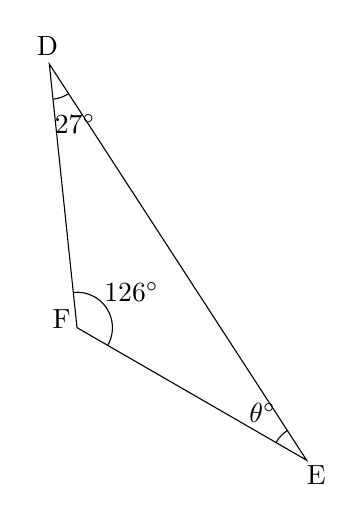
\begin{tikzpicture}[scale=1.5, baseline=(current bounding box.north)]
      \pgfmathsetmacro{\angleA}{27}
      \pgfmathsetmacro{\angleB}{27}
      \pgfmathsetmacro{\angleC}{126}
      \pgfmathsetmacro{\sideC}{4}
      \pgfmathsetmacro{\rotationAngle}{123}
  
    
      \begin{scope}[rotate=\rotationAngle]
        \coordinate (A) at (0,0);
        \coordinate (B) at (\sideC,0);
        \coordinate (C) at (intersection cs: first line={(A)--($(A)+(\angleA:4cm)$)}, second line={(B)--($(B)+(180-\angleB:4cm)$)});
        \draw (A) -- (B) -- (C) -- cycle;
        
        % Mark angles with arcs
        \draw ($(A)!0.3cm!(B)$) arc [start angle=0, end angle=\angleA, radius=0.3cm];
        \draw ($(B)!0.3cm!(C)$) arc [start angle=180-\angleB, end angle=180, radius=0.3cm];
        \draw ($(C)!0.3cm!(A)$) arc [start angle=180+\angleA, end angle=360-\angleB, radius=0.3cm];
        
        % Label angles
        \node at ($(A)!-0.15cm!(B)$) {E};
        \node at ($(B)!-0.15cm!(C)$) {D};
        \node at ($(C)!-0.15cm!(A)$) {F};
        
        % Mark angles in degrees
        \coordinate (midBC) at ($(B)!0.5!(C)$);
        \node at ($(A)!0.55cm!(midBC)$) {$\theta ^\circ$};
    
        \coordinate (midAC) at ($(A)!0.5!(C)$);
        \node at ($(B)!0.55cm!(midAC)$) {27$^\circ$};
    
        \coordinate (midAB) at ($(A)!0.5!(B)$);
        \node at ($(C)!0.55cm!(midAB)$) {126$^\circ$};
      
      \end{scope}
    \end{tikzpicture}
\end{minipage}%
\hfill
\begin{minipage}{0.4\textwidth}
    \begin{align*}
      \angle \text{E} &= 180^\circ - (\angle \text{D} + \angle \text{F}) \\
        &= 180^\circ - (\dotuline{~~~~~~~}^\circ + \dotuline{~~~~~~~}^\circ) \\
        &= 180^\circ - \dotuline{~~~~~~~}^\circ \\
        &= \dotuline{~~~~~~~}^\circ
    \end{align*}
\end{minipage}

\vspace{1cm}\begin{minipage}{0.55\textwidth}
  \refstepcounter{minipagecount}
  \noindent{(\theminipagecount)}\quad
  \begin{tikzpicture}[scale=1.5, baseline=(current bounding box.north)]
      \pgfmathsetmacro{\angleA}{44}
      \pgfmathsetmacro{\angleB}{59}
      \pgfmathsetmacro{\angleC}{77}
      \pgfmathsetmacro{\sideC}{3}
      \pgfmathsetmacro{\rotationAngle}{201}
  
    
      \begin{scope}[rotate=\rotationAngle]
        \coordinate (A) at (0,0);
        \coordinate (B) at (\sideC,0);
        \coordinate (C) at (intersection cs: first line={(A)--($(A)+(\angleA:4cm)$)}, second line={(B)--($(B)+(180-\angleB:4cm)$)});
        \draw (A) -- (B) -- (C) -- cycle;
        
        % Mark angles with arcs
        \draw ($(A)!0.3cm!(B)$) arc [start angle=0, end angle=\angleA, radius=0.3cm];
        \draw ($(B)!0.3cm!(C)$) arc [start angle=180-\angleB, end angle=180, radius=0.3cm];
        \draw ($(C)!0.3cm!(A)$) arc [start angle=180+\angleA, end angle=360-\angleB, radius=0.3cm];
        
        % Label angles
        \node at ($(A)!-0.15cm!(B)$) {Y};
        \node at ($(B)!-0.15cm!(C)$) {Z};
        \node at ($(C)!-0.15cm!(A)$) {X};
        
        % Mark angles in degrees
        \coordinate (midBC) at ($(B)!0.5!(C)$);
        \node at ($(A)!0.55cm!(midBC)$) {$\theta ^\circ$};
    
        \coordinate (midAC) at ($(A)!0.5!(C)$);
        \node at ($(B)!0.55cm!(midAC)$) {59$^\circ$};
    
        \coordinate (midAB) at ($(A)!0.5!(B)$);
        \node at ($(C)!0.55cm!(midAB)$) {77$^\circ$};
      
      \end{scope}
    \end{tikzpicture}
\end{minipage}%
\hfill
\begin{minipage}{0.4\textwidth}
    \begin{align*}
      \angle \text{Y} &= 180^\circ - (\angle \text{Z} + \angle \text{X}) \\
        &= 180^\circ - (\dotuline{~~~~~~~}^\circ + \dotuline{~~~~~~~}^\circ) \\
        &= 180^\circ - \dotuline{~~~~~~~}^\circ \\
        &= \dotuline{~~~~~~~}^\circ
    \end{align*}
\end{minipage}

\vspace{1cm}\begin{minipage}{0.55\textwidth}
  \refstepcounter{minipagecount}
  \noindent{(\theminipagecount)}\quad
  \begin{tikzpicture}[scale=1.5, baseline=(current bounding box.north)]
      \pgfmathsetmacro{\angleA}{26}
      \pgfmathsetmacro{\angleB}{50}
      \pgfmathsetmacro{\angleC}{104}
      \pgfmathsetmacro{\sideC}{4}
      \pgfmathsetmacro{\rotationAngle}{288}
  
    
      \begin{scope}[rotate=\rotationAngle]
        \coordinate (A) at (0,0);
        \coordinate (B) at (\sideC,0);
        \coordinate (C) at (intersection cs: first line={(A)--($(A)+(\angleA:4cm)$)}, second line={(B)--($(B)+(180-\angleB:4cm)$)});
        \draw (A) -- (B) -- (C) -- cycle;
        
        % Mark angles with arcs
        \draw ($(A)!0.3cm!(B)$) arc [start angle=0, end angle=\angleA, radius=0.3cm];
        \draw ($(B)!0.3cm!(C)$) arc [start angle=180-\angleB, end angle=180, radius=0.3cm];
        \draw ($(C)!0.3cm!(A)$) arc [start angle=180+\angleA, end angle=360-\angleB, radius=0.3cm];
        
        % Label angles
        \node at ($(A)!-0.15cm!(B)$) {T};
        \node at ($(B)!-0.15cm!(C)$) {R};
        \node at ($(C)!-0.15cm!(A)$) {S};
        
        % Mark angles in degrees
        \coordinate (midBC) at ($(B)!0.5!(C)$);
        \node at ($(A)!0.55cm!(midBC)$) {$\theta ^\circ$};
    
        \coordinate (midAC) at ($(A)!0.5!(C)$);
        \node at ($(B)!0.55cm!(midAC)$) {50$^\circ$};
    
        \coordinate (midAB) at ($(A)!0.5!(B)$);
        \node at ($(C)!0.55cm!(midAB)$) {104$^\circ$};
      
      \end{scope}
    \end{tikzpicture}
\end{minipage}%
\hfill
\begin{minipage}{0.4\textwidth}
    \begin{align*}
      \angle \text{T} &= 180^\circ - (\angle \text{R} + \angle \text{S}) \\
        &= 180^\circ - (\dotuline{~~~~~~~}^\circ + \dotuline{~~~~~~~}^\circ) \\
        &= 180^\circ - \dotuline{~~~~~~~}^\circ \\
        &= \dotuline{~~~~~~~}^\circ
    \end{align*}
\end{minipage}

\vspace{1cm}\begin{minipage}{0.55\textwidth}
  \refstepcounter{minipagecount}
  \noindent{(\theminipagecount)}\quad
  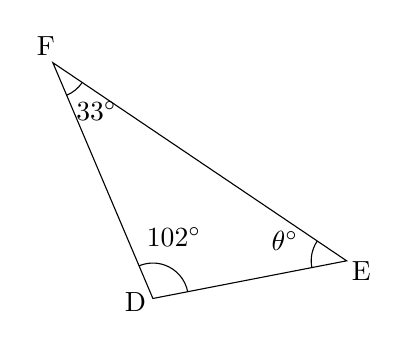
\begin{tikzpicture}[scale=1.5, baseline=(current bounding box.north)]
      \pgfmathsetmacro{\angleA}{45}
      \pgfmathsetmacro{\angleB}{33}
      \pgfmathsetmacro{\angleC}{102}
      \pgfmathsetmacro{\sideC}{3}
      \pgfmathsetmacro{\rotationAngle}{146}
  
    
      \begin{scope}[rotate=\rotationAngle]
        \coordinate (A) at (0,0);
        \coordinate (B) at (\sideC,0);
        \coordinate (C) at (intersection cs: first line={(A)--($(A)+(\angleA:4cm)$)}, second line={(B)--($(B)+(180-\angleB:4cm)$)});
        \draw (A) -- (B) -- (C) -- cycle;
        
        % Mark angles with arcs
        \draw ($(A)!0.3cm!(B)$) arc [start angle=0, end angle=\angleA, radius=0.3cm];
        \draw ($(B)!0.3cm!(C)$) arc [start angle=180-\angleB, end angle=180, radius=0.3cm];
        \draw ($(C)!0.3cm!(A)$) arc [start angle=180+\angleA, end angle=360-\angleB, radius=0.3cm];
        
        % Label angles
        \node at ($(A)!-0.15cm!(B)$) {E};
        \node at ($(B)!-0.15cm!(C)$) {F};
        \node at ($(C)!-0.15cm!(A)$) {D};
        
        % Mark angles in degrees
        \coordinate (midBC) at ($(B)!0.5!(C)$);
        \node at ($(A)!0.55cm!(midBC)$) {$\theta ^\circ$};
    
        \coordinate (midAC) at ($(A)!0.5!(C)$);
        \node at ($(B)!0.55cm!(midAC)$) {33$^\circ$};
    
        \coordinate (midAB) at ($(A)!0.5!(B)$);
        \node at ($(C)!0.55cm!(midAB)$) {102$^\circ$};
      
      \end{scope}
    \end{tikzpicture}
\end{minipage}%
\hfill
\begin{minipage}{0.4\textwidth}
    \begin{align*}
      \angle \text{E} &= 180^\circ - (\angle \text{F} + \angle \text{D}) \\
        &= 180^\circ - (\dotuline{~~~~~~~}^\circ + \dotuline{~~~~~~~}^\circ) \\
        &= 180^\circ - \dotuline{~~~~~~~}^\circ \\
        &= \dotuline{~~~~~~~}^\circ
    \end{align*}
\end{minipage}

\vspace{1cm}\begin{minipage}{0.55\textwidth}
  \refstepcounter{minipagecount}
  \noindent{(\theminipagecount)}\quad
  \begin{tikzpicture}[scale=1.5, baseline=(current bounding box.north)]
      \pgfmathsetmacro{\angleA}{62}
      \pgfmathsetmacro{\angleB}{56}
      \pgfmathsetmacro{\angleC}{62}
      \pgfmathsetmacro{\sideC}{4}
      \pgfmathsetmacro{\rotationAngle}{214}
  
    
      \begin{scope}[rotate=\rotationAngle]
        \coordinate (A) at (0,0);
        \coordinate (B) at (\sideC,0);
        \coordinate (C) at (intersection cs: first line={(A)--($(A)+(\angleA:4cm)$)}, second line={(B)--($(B)+(180-\angleB:4cm)$)});
        \draw (A) -- (B) -- (C) -- cycle;
        
        % Mark angles with arcs
        \draw ($(A)!0.3cm!(B)$) arc [start angle=0, end angle=\angleA, radius=0.3cm];
        \draw ($(B)!0.3cm!(C)$) arc [start angle=180-\angleB, end angle=180, radius=0.3cm];
        \draw ($(C)!0.3cm!(A)$) arc [start angle=180+\angleA, end angle=360-\angleB, radius=0.3cm];
        
        % Label angles
        \node at ($(A)!-0.15cm!(B)$) {R};
        \node at ($(B)!-0.15cm!(C)$) {S};
        \node at ($(C)!-0.15cm!(A)$) {T};
        
        % Mark angles in degrees
        \coordinate (midBC) at ($(B)!0.5!(C)$);
        \node at ($(A)!0.55cm!(midBC)$) {$\theta ^\circ$};
    
        \coordinate (midAC) at ($(A)!0.5!(C)$);
        \node at ($(B)!0.55cm!(midAC)$) {56$^\circ$};
    
        \coordinate (midAB) at ($(A)!0.5!(B)$);
        \node at ($(C)!0.55cm!(midAB)$) {62$^\circ$};
      
      \end{scope}
    \end{tikzpicture}
\end{minipage}%
\hfill
\begin{minipage}{0.4\textwidth}
    \begin{align*}
      \angle \text{R} &= 180^\circ - (\angle \text{S} + \angle \text{T}) \\
        &= 180^\circ - (\dotuline{~~~~~~~}^\circ + \dotuline{~~~~~~~}^\circ) \\
        &= 180^\circ - \dotuline{~~~~~~~}^\circ \\
        &= \dotuline{~~~~~~~}^\circ
    \end{align*}
\end{minipage}

\vspace{1cm}\begin{minipage}{0.55\textwidth}
  \refstepcounter{minipagecount}
  \noindent{(\theminipagecount)}\quad
  \begin{tikzpicture}[scale=1.5, baseline=(current bounding box.north)]
      \pgfmathsetmacro{\angleA}{55}
      \pgfmathsetmacro{\angleB}{61}
      \pgfmathsetmacro{\angleC}{64}
      \pgfmathsetmacro{\sideC}{3}
      \pgfmathsetmacro{\rotationAngle}{34}
  
    
      \begin{scope}[rotate=\rotationAngle]
        \coordinate (A) at (0,0);
        \coordinate (B) at (\sideC,0);
        \coordinate (C) at (intersection cs: first line={(A)--($(A)+(\angleA:4cm)$)}, second line={(B)--($(B)+(180-\angleB:4cm)$)});
        \draw (A) -- (B) -- (C) -- cycle;
        
        % Mark angles with arcs
        \draw ($(A)!0.3cm!(B)$) arc [start angle=0, end angle=\angleA, radius=0.3cm];
        \draw ($(B)!0.3cm!(C)$) arc [start angle=180-\angleB, end angle=180, radius=0.3cm];
        \draw ($(C)!0.3cm!(A)$) arc [start angle=180+\angleA, end angle=360-\angleB, radius=0.3cm];
        
        % Label angles
        \node at ($(A)!-0.15cm!(B)$) {F};
        \node at ($(B)!-0.15cm!(C)$) {D};
        \node at ($(C)!-0.15cm!(A)$) {E};
        
        % Mark angles in degrees
        \coordinate (midBC) at ($(B)!0.5!(C)$);
        \node at ($(A)!0.55cm!(midBC)$) {$\theta ^\circ$};
    
        \coordinate (midAC) at ($(A)!0.5!(C)$);
        \node at ($(B)!0.55cm!(midAC)$) {61$^\circ$};
    
        \coordinate (midAB) at ($(A)!0.5!(B)$);
        \node at ($(C)!0.55cm!(midAB)$) {64$^\circ$};
      
      \end{scope}
    \end{tikzpicture}
\end{minipage}%
\hfill
\begin{minipage}{0.4\textwidth}
    \begin{align*}
      \angle \text{F} &= 180^\circ - (\angle \text{D} + \angle \text{E}) \\
        &= 180^\circ - (\dotuline{~~~~~~~}^\circ + \dotuline{~~~~~~~}^\circ) \\
        &= 180^\circ - \dotuline{~~~~~~~}^\circ \\
        &= \dotuline{~~~~~~~}^\circ
    \end{align*}
\end{minipage}

\vspace{1cm}\begin{minipage}{0.55\textwidth}
  \refstepcounter{minipagecount}
  \noindent{(\theminipagecount)}\quad
  \begin{tikzpicture}[scale=1.5, baseline=(current bounding box.north)]
      \pgfmathsetmacro{\angleA}{63}
      \pgfmathsetmacro{\angleB}{49}
      \pgfmathsetmacro{\angleC}{68}
      \pgfmathsetmacro{\sideC}{3}
      \pgfmathsetmacro{\rotationAngle}{72}
  
    
      \begin{scope}[rotate=\rotationAngle]
        \coordinate (A) at (0,0);
        \coordinate (B) at (\sideC,0);
        \coordinate (C) at (intersection cs: first line={(A)--($(A)+(\angleA:4cm)$)}, second line={(B)--($(B)+(180-\angleB:4cm)$)});
        \draw (A) -- (B) -- (C) -- cycle;
        
        % Mark angles with arcs
        \draw ($(A)!0.3cm!(B)$) arc [start angle=0, end angle=\angleA, radius=0.3cm];
        \draw ($(B)!0.3cm!(C)$) arc [start angle=180-\angleB, end angle=180, radius=0.3cm];
        \draw ($(C)!0.3cm!(A)$) arc [start angle=180+\angleA, end angle=360-\angleB, radius=0.3cm];
        
        % Label angles
        \node at ($(A)!-0.15cm!(B)$) {L};
        \node at ($(B)!-0.15cm!(C)$) {N};
        \node at ($(C)!-0.15cm!(A)$) {M};
        
        % Mark angles in degrees
        \coordinate (midBC) at ($(B)!0.5!(C)$);
        \node at ($(A)!0.55cm!(midBC)$) {$\theta ^\circ$};
    
        \coordinate (midAC) at ($(A)!0.5!(C)$);
        \node at ($(B)!0.55cm!(midAC)$) {49$^\circ$};
    
        \coordinate (midAB) at ($(A)!0.5!(B)$);
        \node at ($(C)!0.55cm!(midAB)$) {68$^\circ$};
      
      \end{scope}
    \end{tikzpicture}
\end{minipage}%
\hfill
\begin{minipage}{0.4\textwidth}
    \begin{align*}
      \angle \text{L} &= 180^\circ - (\angle \text{N} + \angle \text{M}) \\
        &= 180^\circ - (\dotuline{~~~~~~~}^\circ + \dotuline{~~~~~~~}^\circ) \\
        &= 180^\circ - \dotuline{~~~~~~~}^\circ \\
        &= \dotuline{~~~~~~~}^\circ
    \end{align*}
\end{minipage}

\vspace{1cm}\begin{minipage}{0.55\textwidth}
  \refstepcounter{minipagecount}
  \noindent{(\theminipagecount)}\quad
  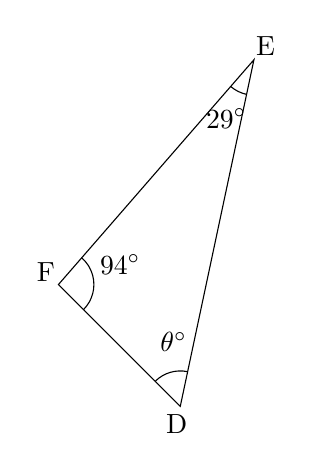
\begin{tikzpicture}[scale=1.5, baseline=(current bounding box.north)]
      \pgfmathsetmacro{\angleA}{57}
      \pgfmathsetmacro{\angleB}{29}
      \pgfmathsetmacro{\angleC}{94}
      \pgfmathsetmacro{\sideC}{3}
      \pgfmathsetmacro{\rotationAngle}{78}
  
    
      \begin{scope}[rotate=\rotationAngle]
        \coordinate (A) at (0,0);
        \coordinate (B) at (\sideC,0);
        \coordinate (C) at (intersection cs: first line={(A)--($(A)+(\angleA:4cm)$)}, second line={(B)--($(B)+(180-\angleB:4cm)$)});
        \draw (A) -- (B) -- (C) -- cycle;
        
        % Mark angles with arcs
        \draw ($(A)!0.3cm!(B)$) arc [start angle=0, end angle=\angleA, radius=0.3cm];
        \draw ($(B)!0.3cm!(C)$) arc [start angle=180-\angleB, end angle=180, radius=0.3cm];
        \draw ($(C)!0.3cm!(A)$) arc [start angle=180+\angleA, end angle=360-\angleB, radius=0.3cm];
        
        % Label angles
        \node at ($(A)!-0.15cm!(B)$) {D};
        \node at ($(B)!-0.15cm!(C)$) {E};
        \node at ($(C)!-0.15cm!(A)$) {F};
        
        % Mark angles in degrees
        \coordinate (midBC) at ($(B)!0.5!(C)$);
        \node at ($(A)!0.55cm!(midBC)$) {$\theta ^\circ$};
    
        \coordinate (midAC) at ($(A)!0.5!(C)$);
        \node at ($(B)!0.55cm!(midAC)$) {29$^\circ$};
    
        \coordinate (midAB) at ($(A)!0.5!(B)$);
        \node at ($(C)!0.55cm!(midAB)$) {94$^\circ$};
      
      \end{scope}
    \end{tikzpicture}
\end{minipage}%
\hfill
\begin{minipage}{0.4\textwidth}
    \begin{align*}
      \angle \text{D} &= 180^\circ - (\angle \text{E} + \angle \text{F}) \\
        &= 180^\circ - (\dotuline{~~~~~~~}^\circ + \dotuline{~~~~~~~}^\circ) \\
        &= 180^\circ - \dotuline{~~~~~~~}^\circ \\
        &= \dotuline{~~~~~~~}^\circ
    \end{align*}
\end{minipage}

\vspace{1cm}

\end{document}
